\section{LFS Server}

\subsection{API}

\paragraph{}
The api of the LFS server is well defined at \url{https://github.com/git-lfs/git-lfs/blob/main/docs/api/batch.md}. From this we can derive a few structures, and some functions that will be needed to create and validate them. 

\paragraph{}
The request and response packages also need some enums to be defined, but as needed by other packages, they will be defined as a sub-package of api. 

\paragraph{}
The repository name is found in the query parameters, so a very simple structure is needed to hold it.

\paragraph{}
Finally, another part of the api required by our system is the stateless proof of access, implemented by a jwt. A structure handle the decoding of the jwt, and another is specific to the payload of the jwt, containing the repo, the write access, and user name. This one is created from the jwt decoding structure.

\begin{figure}[H]
    \centering
    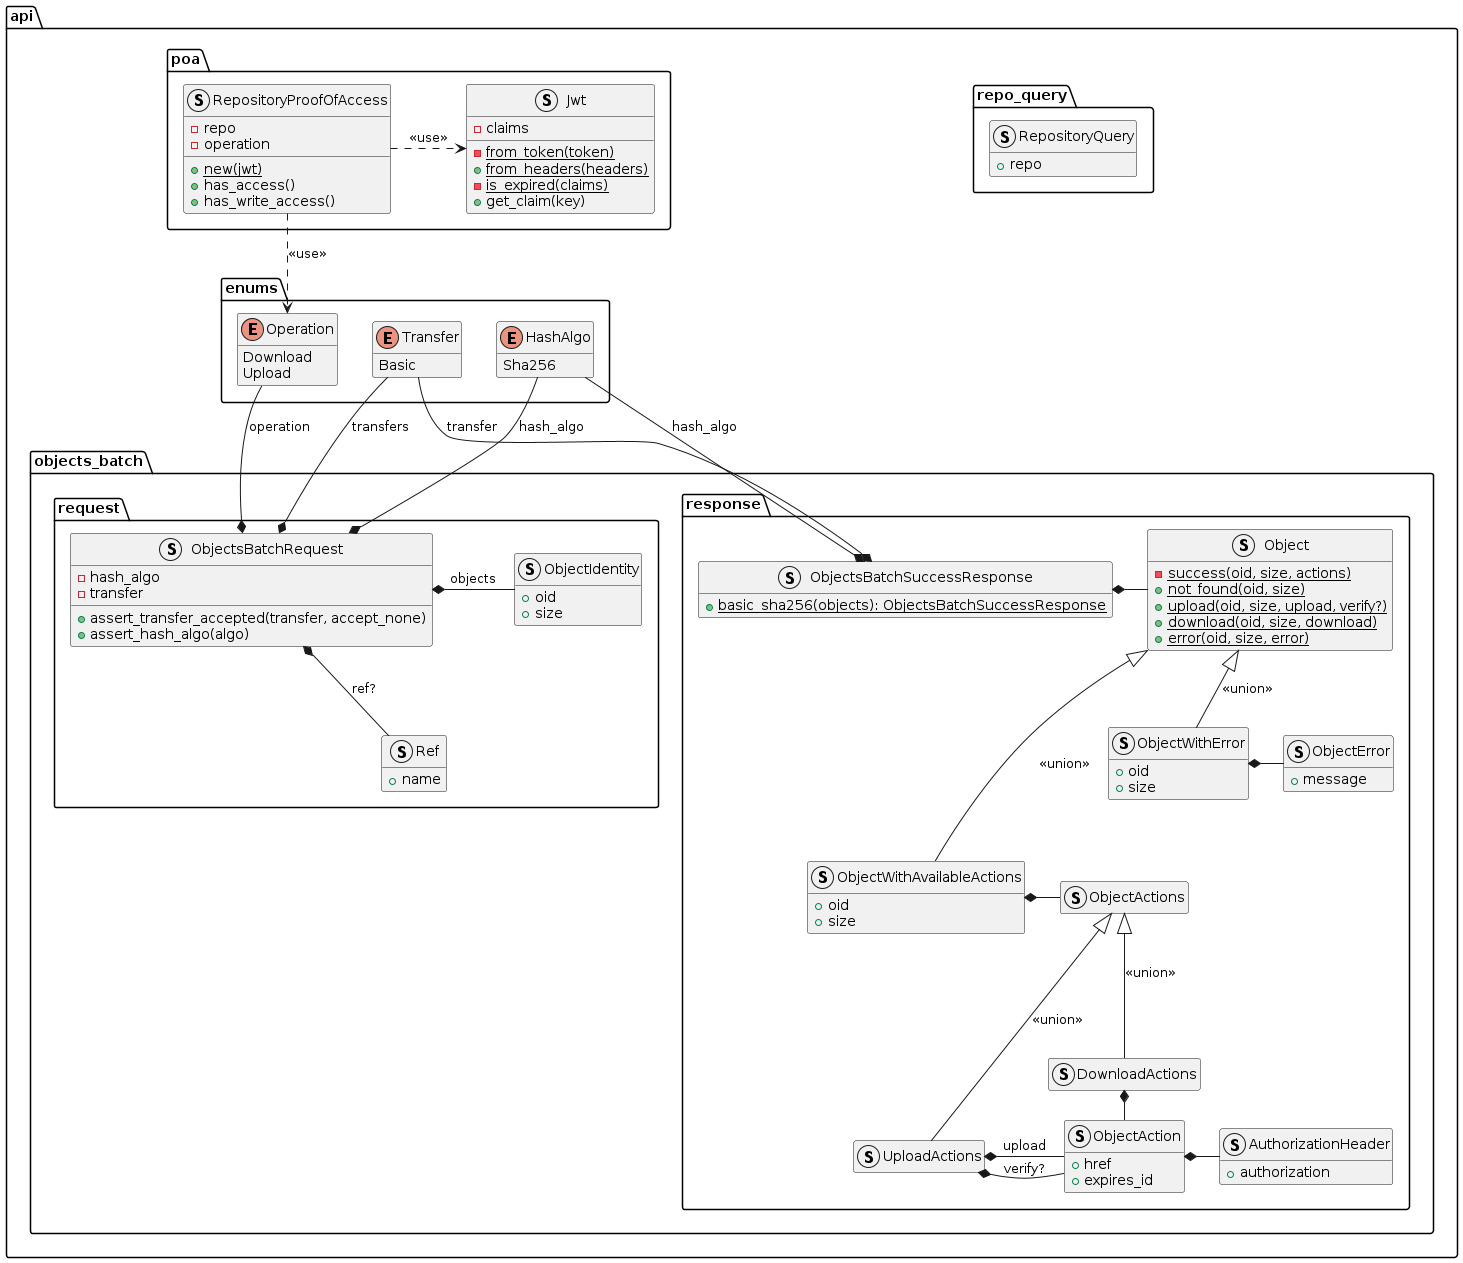
\includegraphics[width=0.9\textwidth]{iteration_03/diagrams/batch_api_structure.png}
    \caption{Objects batch  API}
    \label{fig:lfs_server_api}
\end{figure}

\subsection{Services}

To implement the api, we need to define a few services. We should be able to access files on a storage (the file system, S3, ...), to sign links to upload or download files, and maybe others in the future. These services should be injected in the server definition, so that we can easily change the implementation of the storage, or the signing strategy (internal, external, ...).

\begin{figure}[H]
    \centering
    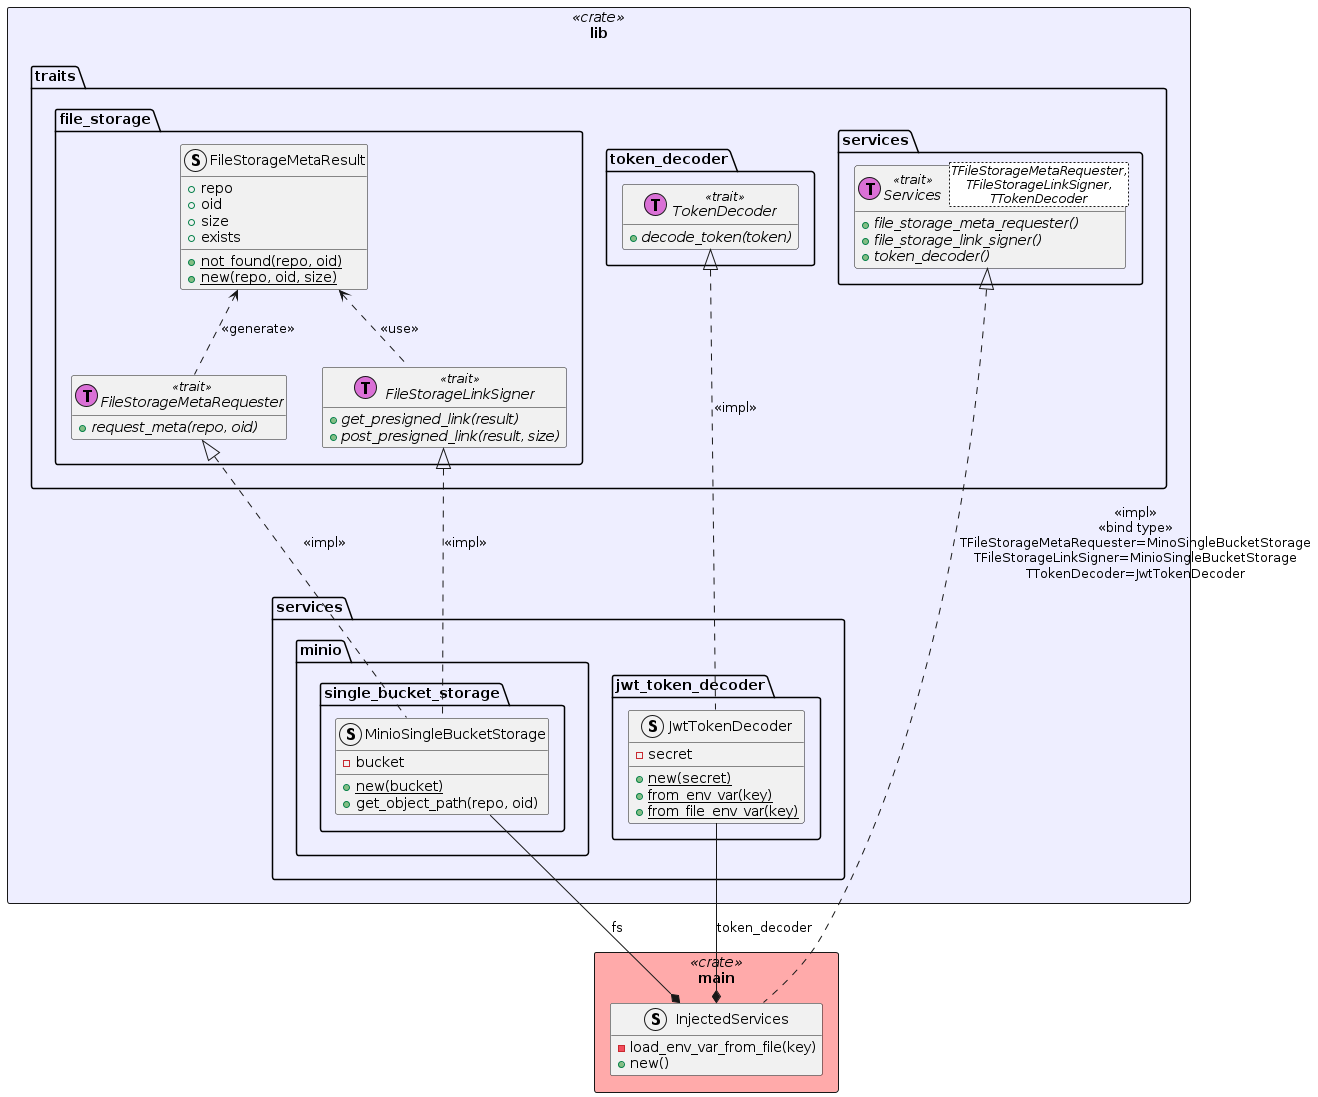
\includegraphics[width=\textwidth]{iteration_03/diagrams/services_injection.png}
    \caption{Service injection}
    \label{fig:services_injection}
\end{figure}

\paragraph{}
To achieve such injection, we make use of the traits feature of rust. The required services, defined in \textit{Services}, are injected. On the other side, we create the structure \textit{MinioSingleBucketStorage}, and implements the traits for it. Finally, the main crate will create a structure \textit{InjectedServices} that will hold the storage implementation, bind the \textit{Services} traits to it, and inject it in the server definition.

\paragraph{}
On the other side, it also make sense to inject the token decoder, so we can chose implementation, especially the fetch of the secret, at the highest level. 
